\documentclass[11pt]{standalone}
\usepackage{amssymb}
\usepackage{amsmath}
\usepackage[no-math]{fontspec}
\usepackage{unicode-math}
\usepackage{libertinus}
\usepackage{pgf,xcolor}
\usepackage{tikz}
\usetikzlibrary{arrows.meta, backgrounds}
\usepackage{pgfplots}
\pgfplotsset{compat=newest}

\definecolor{my_darkgray}{HTML}{484949}
\definecolor{my_lightgray}{HTML}{F3F4F4}
\definecolor{my_darkblue}{HTML}{005A94}
\definecolor{my_lightblue}{HTML}{CCDEE9}
\definecolor{my_yellow}{HTML}{FFEC7F}
\definecolor{my_red}{HTML}{E60000}
\definecolor{my_orange}{HTML}{E87846}

\begin{document}
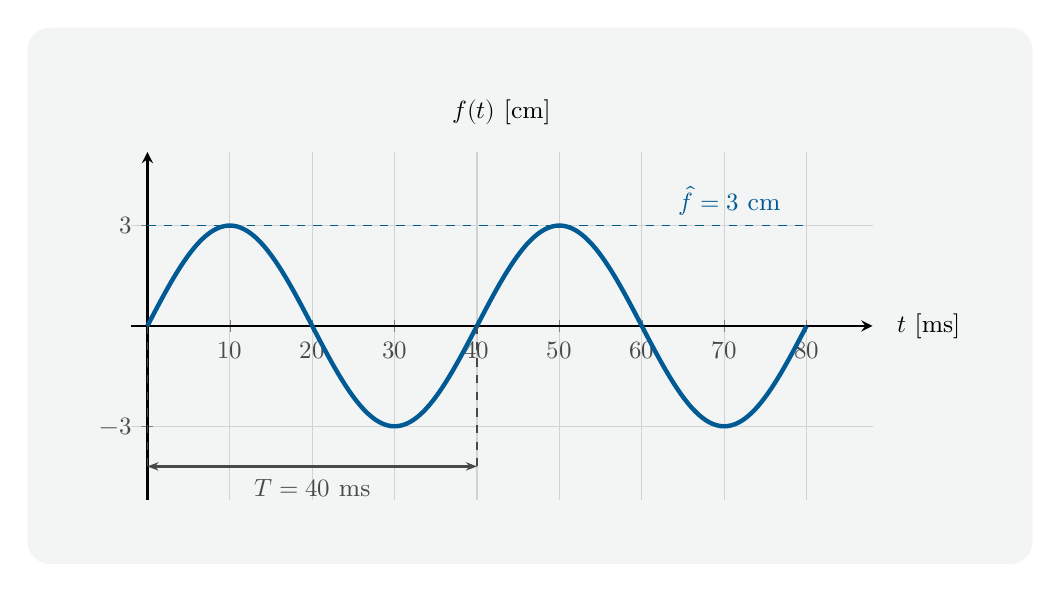
\begin{tikzpicture}[
    show background rectangle,
    background rectangle/.style={fill=my_lightgray, rounded corners=8pt},
    inner frame sep=0.8cm
]

\begin{axis}[
    axis lines = center,
    xlabel = {$t$ [ms]},
    ylabel = {$f(t)$ [cm]},
    xlabel style={at={(axis description cs:1.02,0.5)}, anchor=west, font=\small},
    ylabel style={at={(axis description cs:0.5,1.05)}, anchor=south, font=\small},
    xmin = -2,
    xmax = 88,
    ymin = -5.2,
    ymax = 5.2,
    xtick = {0, 10, 20, 30, 40, 50, 60, 70, 80},
    ytick = {-3, 0, 3},
    yticklabels = {$-3$, $0$, $3$},
    axis line style = {thick},
    grid = both,
    grid style = {draw=my_lightgray!60!white, line width=0.4pt},
    major grid style = {draw=my_lightgray!80!my_darkgray, line width=0.5pt},
    tick label style = {font=\small, color=my_darkgray},
    width = 11cm,
    height = 6cm,
    % axis equal not used: time axis (ms) vs displacement (cm) have different units
]

%% Main curve: f(t) = 3*sin(50*pi*t [s]) = 3*sin(50*pi * t/1000 [ms])
%% = 3*sin(pi*t/20) with t in ms
\addplot[
    draw = my_darkblue,
    samples = 300,
    ultra thick,
    domain = 0:80,
]{ 3*sin(deg(pi*x/20)) };

%% --- Amplitude annotation ---
% Vertical brace / arrow indicating amplitude on the right side of the plot
% Dashed line at y = 3
\addplot[
    draw = my_darkblue,
    dashed,
    thin,
    domain = 0:80,
]{ 3 };

% Label for amplitude: placed inside the plot, above the dashed line
\node[anchor=south east, font=\small, color=my_darkblue]
    at (axis cs: 78, 3) {$\hat{f} = 3~\text{cm}$};

%% --- Period annotation: double-headed arrow from t=0 to t=40 ms ---
% Horizontal arrow below the curve
\draw[{Stealth[length=4pt]}-{Stealth[length=4pt]}, thick, color=my_darkgray]
    (axis cs: 0, -4.2) -- (axis cs: 40, -4.2);

\node[anchor=north, font=\small, color=my_darkgray]
    at (axis cs: 20, -4.3) {$T = 40~\text{ms}$};

% Thin vertical dashed guide lines for the period arrow
\draw[dashed, thin, color=my_darkgray]
    (axis cs: 0, -4.2) -- (axis cs: 0, 0);
\draw[dashed, thin, color=my_darkgray]
    (axis cs: 40, -4.2) -- (axis cs: 40, 0);

\end{axis}

\end{tikzpicture}
\end{document}
